\documentclass[tikz, margin=2]{standalone}
\usepackage{amsmath}


\begin{document}
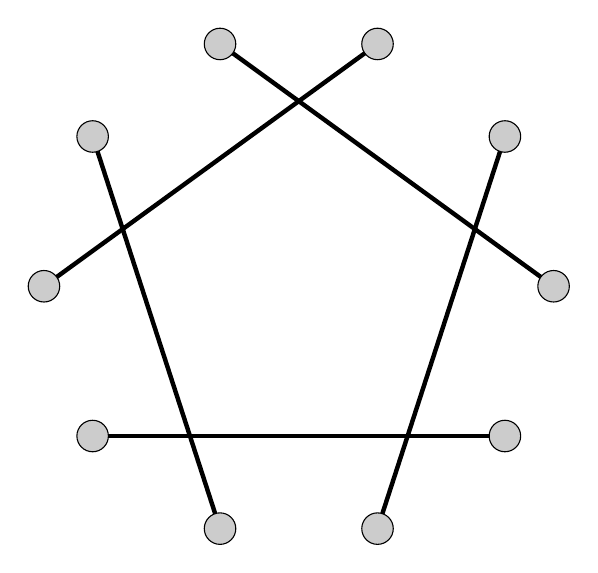
\begin{tikzpicture}

% Draw the edges
\draw[ultra thick] (0,0) -- (-1.618,4.980);
\draw[ultra thick] (-2.236,3.078) -- (2,6.155);
\draw[ultra thick] (0,6.155) -- (4.236,3.078);
\draw[ultra thick] (3.618,4.980) -- (2,0);
\draw[ultra thick] (3.618,1.176) -- (-1.618,1.176);

% Draw the nodes
\filldraw[color=black,fill=gray!40] (0,0) circle (.2);
\filldraw[color=black,fill=gray!40] (-1.618,1.176) circle (.2);
\filldraw[color=black,fill=gray!40] (-2.236,3.078) circle (.2);
\filldraw[color=black,fill=gray!40] (-1.618,4.980) circle (.2);
\filldraw[color=black,fill=gray!40] (0,6.155) circle (.2);
\filldraw[color=black,fill=gray!40] (2,6.155) circle (.2);
\filldraw[color=black,fill=gray!40] (3.618,4.980) circle (.2);
\filldraw[color=black,fill=gray!40] (4.236,3.078) circle (.2);
\filldraw[color=black,fill=gray!40] (3.618,1.176) circle (.2);
\filldraw[color=black,fill=gray!40] (2,0) circle (.2);

\end{tikzpicture}
\end{document}
